\documentclass[10pt]{beamer}

\usepackage{natbib}

\usetheme[progressbar=frametitle]{metropolis}
\usepackage{appendixnumberbeamer}

\usepackage{booktabs}
\usepackage[scale=2]{ccicons}

\usepackage{pgfplots}
\usepgfplotslibrary{dateplot}

\usepackage{xspace}
\newcommand{\themename}{\textbf{\textsc{metropolis}}\xspace}

\usepackage{amsmath, bm}
\usepackage[ruled,vlined]{algorithm2e}
\usepackage[utf8]{inputenc}



\title{Generative Adversarial Networks}
\subtitle{}
% \date{\today}
\date{}
\author{Davi Barreira}
\institute{FGV - Escola de Matemática Aplicada}
% \titlegraphic{\hfill\includegraphics[height=1.5cm]{logo.pdf}}
\usepackage{caption}
\captionsetup[figure]{font=footnotesize}

\begin{document}

\maketitle

\begin{frame}{Table of contents}
  \setbeamertemplate{section in toc}[sections numbered]
  \tableofcontents[hideallsubsections]
\end{frame}

\AtBeginSection{}
\section[Introdução]{Introdução}
\begin{frame}[fragile]{Introdução}

	\textbf{Generative Adversarial Networks} (GAN)
	foram originalmente introduzidas por \citet{goodfellow2014}.
	Essas redes são utilizadas com o objetivo de gerar
	dados sintéticos realísticos a partir de dados reais.

    \begin{figure}[H]
        \centering
        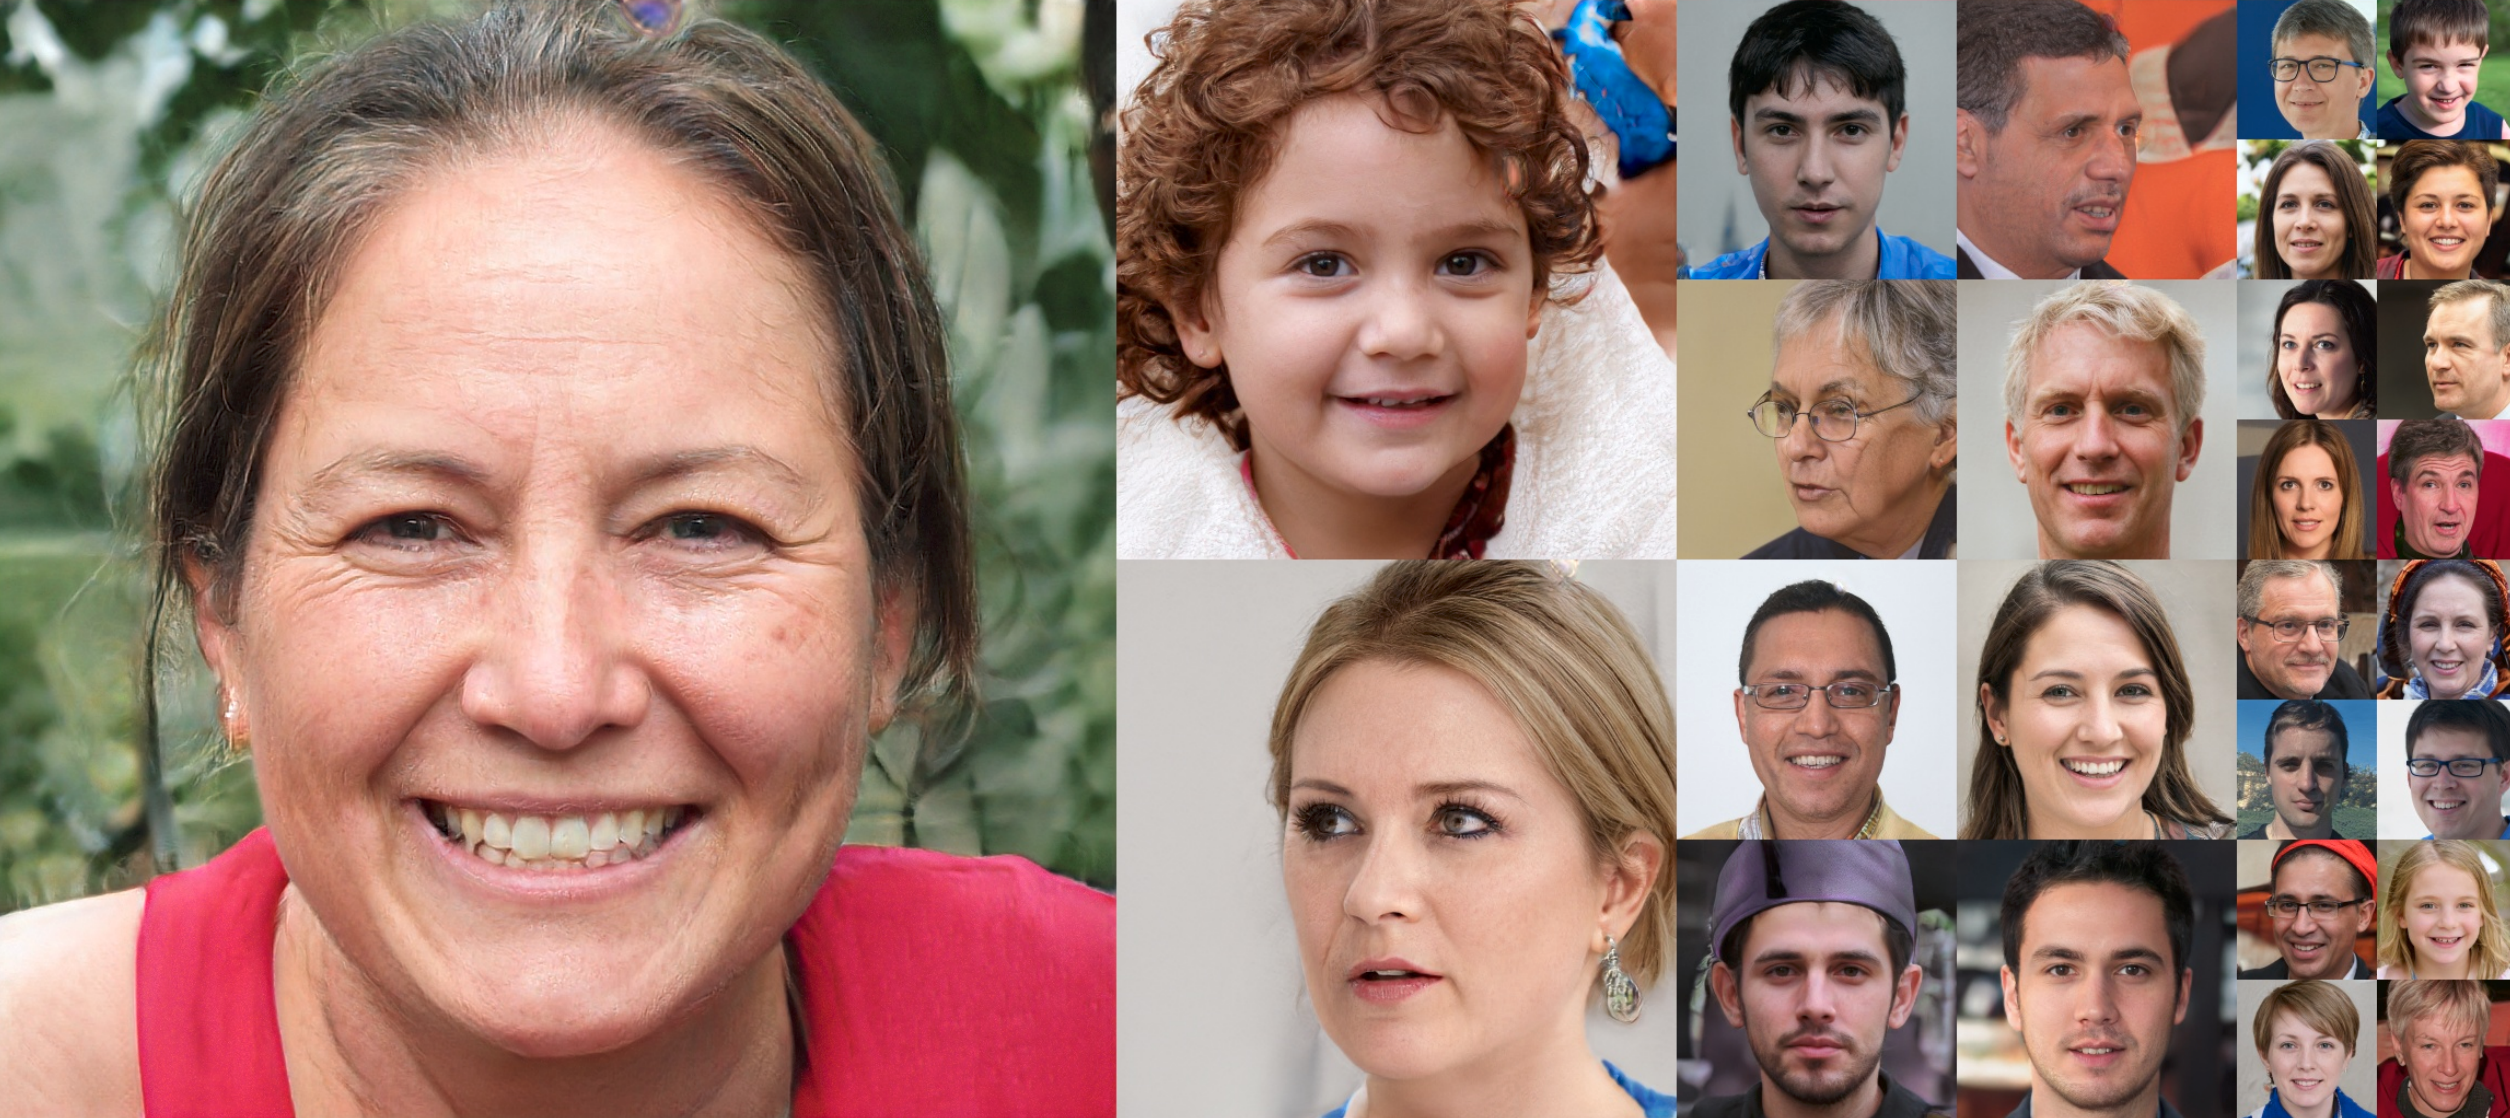
\includegraphics[width=6cm]{images/gans-faces.png}
        \caption{Faces geradas por GAN
        \footnote{https://towardsdatascience.com/generating-modern-arts-using-generative-adversarial-network-gan-on-spell-39f67f83c7b4}.}
    \end{figure}

\end{frame}

\begin{frame}[fragile]{Introdução}

	A geração de novas amostras sintéticas tem diferentes utilidades,
	como aprendizado semi-supervisionado, geração de exemplos
	adversariais, \textit{style transfer}, entre outros.

    \begin{figure}[H]
        \centering
        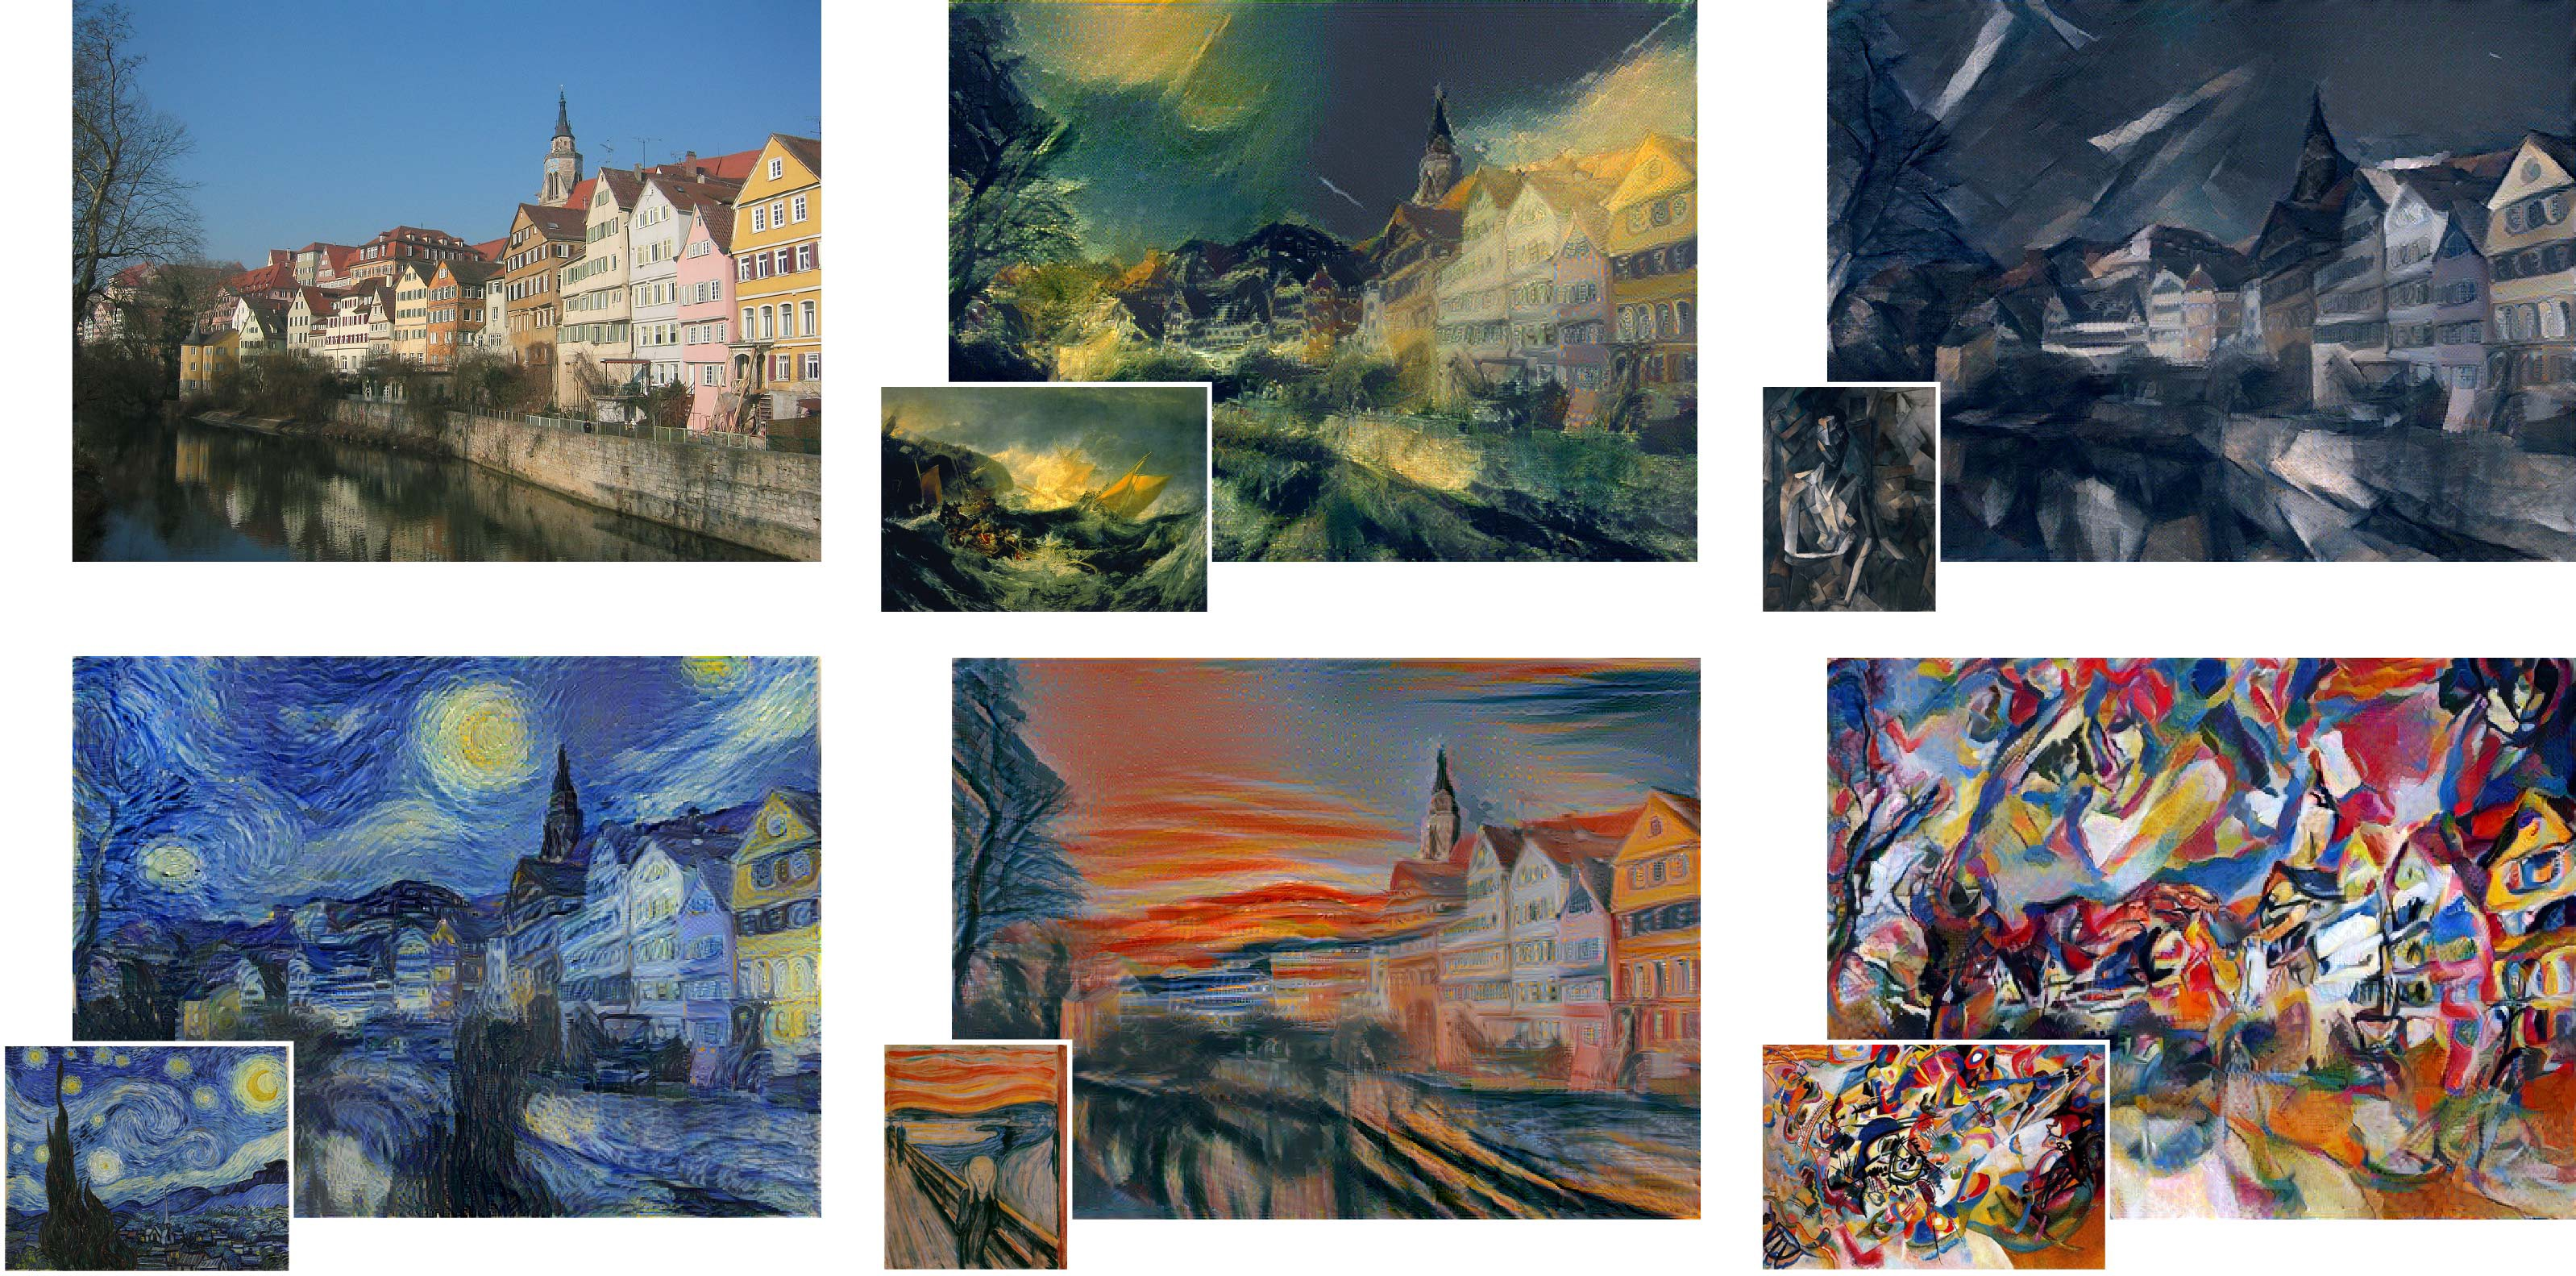
\includegraphics[width=6cm]{images/style-transfer.jpeg}
        \caption{Style transfer utilizando CycleGan
        \footnote{https://towardsdatascience.com/style-transfer-with-gans-on-hd-images-88e8efcf3716}.}
    \end{figure}


\end{frame}

\begin{frame}[fragile]{Introdução}

	A ideia geral por trás das GANs é utilizar duas redes neurais
	competindo uma com a outra, sendo uma rede responsável por
	gerar amostras parecidas com os dados reais (\textit{gerador})
	, enquanto a outra
	busca identificar quando o dado é real ou sintético
	(\textit{descriminador}).

    \begin{figure}[H]
        \centering
        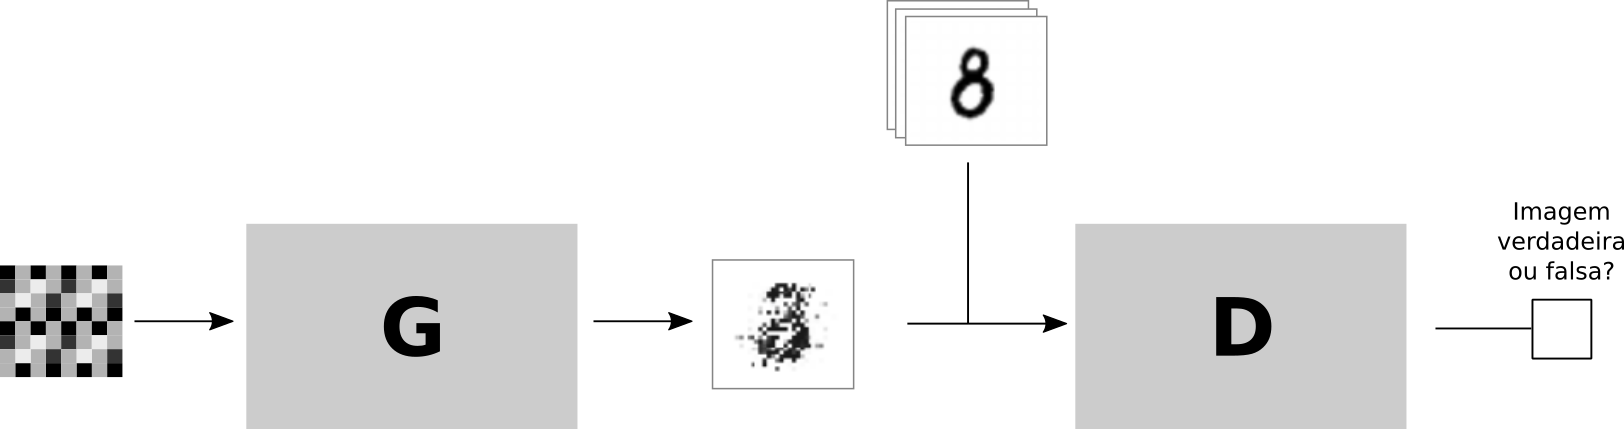
\includegraphics[width=10cm]{images/gan_scheme.png}
        \caption{Desenho esquemático de uma GAN "convencional".}
    \end{figure}

\end{frame}

\AtBeginSection{}
\section[Teoria]{Formalização Teórica}
\begin{frame}[fragile]{Formalização Teórica}
	Na formalização teórica da modelagem das 
	redes adversariais, consideraremos que
	o gerador e o descriminador são ambos \textit{multilayer perceptrons}.
	Os dados reais possuem uma distrbuição
	$p_{data}(\bm x)$, enquanto $p_g$ é a distribuição do gerador e
	$p_z(\bm z)$ é a priori do ruído de entrada. A função
	$G(\bm z, \theta_g)$ é a função diferenciável que transforma $\bm z$ no
	dado sintético, onde $\theta_g$ são os parâmetros da rede.
	A função $D(\bm x, \theta_d)$ retorna a probabilidade de $\bm x$ ter
	sido amostrada de $p_{data}$ invés de $p_g$.
	\begin{itemize}
		\item $p_g$ - Distribuição dos dados sintéticos;
		\item $p_z$ - Distribuição priori dos rúidos de entrada;
		\item $p_{data}$ - Distribuição real dos dados;
		\item $G(\bm z,\theta_g)$ - Função geradora;
		\item $D(\bm x,\theta_d)$ - Função discriminadora.
	\end{itemize}
\end{frame}


\begin{frame}[fragile]{Formalização Teórica}
	
	Nós treinamos $D$ buscando maximizar
	a capacidade de discernir dados de $p_{data}$ de $p_g$. Ao
	mesmo tempo que treinamos $G$ para minimizar $log(1-D(G(\bm z)))$.
	O treino da rede se resume ao problema de otimização dado
	pela seguinte função objetivo:
	\small
    $$
    \min_{G} \max_D V(D,G) =
    \mathbb{E}_{x\sim p_{data}(\bm x)}\left[\log{(D(\bm x))}\right]+
    \mathbb{E}_{z\sim p_z(\bm z)}\left[1-\log{(D(G(\bm z)))}\right]
    $$

    \begin{figure}[H]
        \centering
        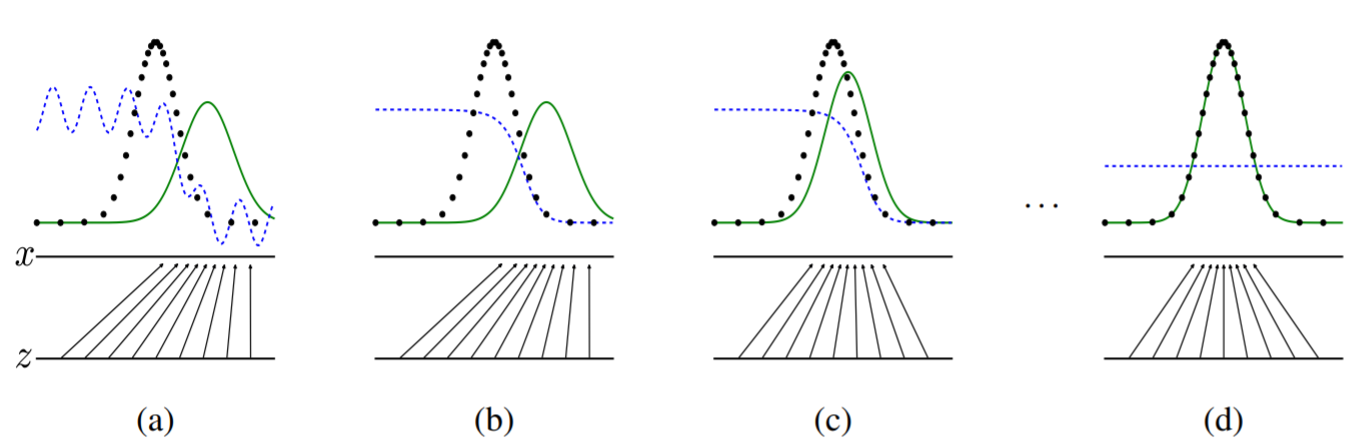
\includegraphics[width=8cm]{images/gan-algorithmscheme.png}
        \caption{De (a) até (d), o desenho ilustra a evolução do
        algoritmo ao ser treinado. A linha azul representa a
        distrbuição do descriminador, a linha verde representa
        a $p_g$, e os pontos pretos representam $p_{data}$
        \footnote{Imagem de \citet{goodfellow2014}}.}
    \end{figure}
	 
\end{frame}

\begin{frame}[fragile]{Formalização Teórica}

  \footnotesize
  \begin{algorithm}[H]
  \SetAlgoLined
  \For{número de iterações de treino}{
  	\For{k passos}{
  		Amostre $m$ valores $\{\bm z^{(1)},...,\bm z^{(m)} \}$
  		da priori $p_z(\bm z)$;

  		Amostre $m$ exemplos $\{\bm x^{(1)},...,\bm x^{(m)} \}$
  		da fução dos dados $p_{data}(\bm x)$;

  		Atualize o \textit{discriminator} utilizando
  		\textit{stochastic gradient descent}:
  		$$
  		\nabla_{\theta_d}\frac{1}{m}\sum^{m}_{i=1}
  		\left[
  		log D(\bm x^{(i)}) + log(1-D(G(\bm z^{(i)})))
  		\right]
  		$$
  	}

	Amostre $m$ valores $\{\bm z^{(1)},...,\bm z^{(m)} \}$
	da priori $p_z(\bm z)$;

	Atualize o \textit{generator} utilizando
	\textit{stochastic gradient descent}:
  		$$
  		\nabla_{\theta_d}\frac{1}{m}\sum^{m}_{i=1}
  		log(1-D(G(\bm z^{(i)})))
  		$$
  }
   \caption{GAN descrita em \citet{goodfellow2014}}
  \end{algorithm}

\end{frame}

\begin{frame}[fragile]{Formalização Teórica}
	
	Vamos estabelecer alguns resultados teóricos do funcionamento
	do algoritmo.

	\small
	\textbf{Proposição 1.} Para G fixo, o discriminador D ótimo é
	$
	D^*_G(\bm x) = \frac{p_{data}(\bm x)}
	{p_{data}(\bm x) + p_g(\bm x)}
	$.

	\hfill
	\break
	\textbf{Teorema 1.} O mínimo global da função objetivo
	é atingido se, e somente se, $p_g = p_{data}$.

	\hfill
	\break
	\textbf{Proposição 2.} Se G e D tiverem capacidade suficiente,
	e, em cada passo do Algortimo 1, o discriminador atingir o seu
	ótimo dado G com $p_g$ sendo atualizado de acordo com
    $$
    \mathbb{E}_{x\sim p_{data}(\bm x)}\left[\log{(D(\bm x))}\right]+
    \mathbb{E}_{z\sim p_z(\bm z)}\left[1-\log{(D(G(\bm z)))}\right]
    $$
    então $p_g$ converge para $p_{data}$.

\end{frame}

\section [Teoria]{Entendendo a Função Objetivo}
\begin{frame}[fragile]{Entendendo a Função Objetivo}
  $$V(D,G)=
    \mathbb{E}_{x\sim p_{data}(\bm x)}\left[\log{(D(\bm x))}\right]+
    \mathbb{E}_{z\sim p_z(\bm z)}\left[1-\log{(D(G(\bm z)))}\right]
  $$
  \pause
  $$= \int_x p_{data}(x)\log{(D(x))}dx + \int_z p_z(z)\log{(1-D(G(z)))}dz $$
  \pause
  $$x = G(z) \rightarrow z = G^{-1}(x) \rightarrow dz = (G^{-1}(x))dx $$
  $$\rightarrow p_g(x) = p_z(G^{-1})(G^{-1})'(x)dx $$
  \pause
  $$= \int_x p_{data}(x)\log{(D(x))}dx + \int_x p_z(G^{-1}(x))\log{(1-D(x))}(G^{-1})'(x)dx $$
  \pause
  $$= \int_x p_{data}(x)\log{(D(x))}dx + \int_x p_g(x)\log{(1-D(x))}dx $$
  \pause
  $$= \int_x p_{data}(x)\log{(D(x))} + p_g(x)\log{(1-D(x))}dx $$
\end{frame}

\begin{frame}[fragile]{Entendendo a Função Objetivo}
 $$\max_{D} V(D,G) = \max_{D}\int_x p_{data}(x)\log{(D(x))} + p_g(x)\log{(1-D(x))}dx $$
 \pause
 $$\frac{\partial}{\partial D(x)} \left(p_{data}(x)\log{(D(x))} + p_g(x)\log{(1-D(x))}\right) = 0 $$
 \pause
 $$\rightarrow \dfrac{p_{data}(x)}{D(x)} - \dfrac{p_g(x)}{1 - D(x)} = 0 $$
 $$\rightarrow D(x) = \dfrac{p_{data}(x)}{p_{data}(x)+p_g(x)} $$
\end{frame}

\begin{frame}[fragile]{Entendendo a Função Objetivo}
 Suponha que o discriminador $D^*_G(x)$ seja ótimo\\
 Então o gerador ótimo produz $p_g(x) = p_{data}(x)$ \\
 $$\rightarrow D^*_G(x) = \dfrac{p_{data}(x)}{p_{data}(x) + p_g(x)}$$
\end{frame}

\begin{frame}[fragile]{Entendendo a Função Objetivo}
  $$C(G) = \max_{D}V(G,D)$$
  \pause
  $$= \max_{D} \int_{x}p_{data}(x)\log{D(x)} + p_{g}\log{1-D(x)}dx $$
  \pause
  $$= \int_{x}p_{data}(x)\log{\left(D_{G}^{*}(x)\right)} + p_{g}(x)\log{\left(1-D_{g}^{*}(x)\right)}dx $$
  \pause
  $$= \int_{x}p_{data}(x)\log{\left(\dfrac{p_{data}(x)}{p_{data}(x) + p_{g}(x)}\right)} + p_{g}(x)\log{\left(\dfrac{p_{data}(x)}{p_{data}(x) + p_{g}(x)}\right)}dx $$
  \pause
  $$= \int_{x}p_{data}(x)\log{\left(\dfrac{p_{data}(x)}{\dfrac{p_{data}(x) + p_{g}(x)}{2}}\right)} + p_{g}(x)\log{\left(\dfrac{p_{data}(x)}{\dfrac{p_{data}(x) + p_{g}(x)}{2}}\right)}dx	$$
  \pause
  $$= KL\left[p_{data}(x)||\dfrac{p_{data}(x)+p_g(x)}{2}\right] + KL\left[p_g(x)||\dfrac{p_{data}(x) + p_g(x)}{2}\right] - \log{4} $$
\end{frame}

\begin{frame}[fragile]{Entendendo a Função Objetivo}
  $$C(G) = KL\left[p_{data}(x)||\frac{p_{data}(x)+p_g(x)}{2}\right] + KL\left[p_g(x)||\frac{p_{data}(x) + p_g(x)}{2}\right] - \log{4}$$
  \pause
  $$\min_G C(G) = 0+0-\log{4} = -\log{4} $$
  $$KL\left[p_{data}(x)||\dfrac{p_{data}(x) + p_g(x)}{2}\right] = 0$$
  \pause
  quando, $p_{data}(x) = \dfrac{p_{data}(x)+p_g(x)}{2}$
  \pause
  $$\rightarrow p_{data}(x) = p_g(x)$$
\end{frame}

\begin{frame}[fragile]{KL (Kullback-Leibler) divergence}
  Jensen-Shannon Divergency (symetric KL):
  $$JSD(P||Q) = \frac{1}{2}D_{KL}(P||M) + \frac{1}{2}D_KL(Q||M),$$
  $$M = \frac{1}{2}(P+Q)$$
\end{frame}

\begin{frame}[fragile]{Resumo:}
  $$V(G,D) = \mathbb{E}_{x~p_{data}(x)}\left[\log{(D(x))}\right]+\mathbb{E}_{z~p_z(x)}\left[1-\log{(D(D(z)))}\right]$$
  Gerador $G$, Discriminador $D$ \\
  Encontro $G^*$, tal que \\
  $$G^* = \arg{\min_G \max_D} V(G,D)$$\\
  Dado $G, \max_{D}V(G,D)$
  $$= -2\log{2} + 2JSD(P_{data}(x)||P_g(x))$$
\end{frame}


\begin{frame}[allowframebreaks]{References}

% \renewcommand{\bibsection}{\section{}}
  \renewcommand{\section}[2]{}%
  \bibliography{gan}
  % \bibliographystyle{plainnat}
  % \bibliographystyle{plain}
  % \bibliographystyle{abbrv}
  \bibliographystyle{apa}

\end{frame}

\end{document}
